%!TEX root = ../main.tex

\section*{Results}

  \subsection*{Mindpipe}

  We have developed mindpipe, a flexible and modular pipeline for 16S data analysis, that allows us to infer co-occurence networks from 16S sequencing data.
  It incorporates various popular, publicly available tools as well as custom Python modules and scripts to facilitate inference of co-occurrence networks from 16S data.
  It enables the user to process 16S sequence data or count matrices using different combinations of the incorporated tools for intermediate analyses as well as inference of co-occurrence networks.
  The pipeline workflow is shown in Figure~\ref{fig:figure1}.
  Each process in the pipeline supports alternate tools for performing the same task, users can use the configuration file to change these values.
  We perform a systematic analysis of each step of the pipeline to determine the set of default options for the pipeline.
  We also provide the users with a set of guidelines to facilitate tool selection as appropriate for their data.


  \begin{figure}[h]
    \centering
    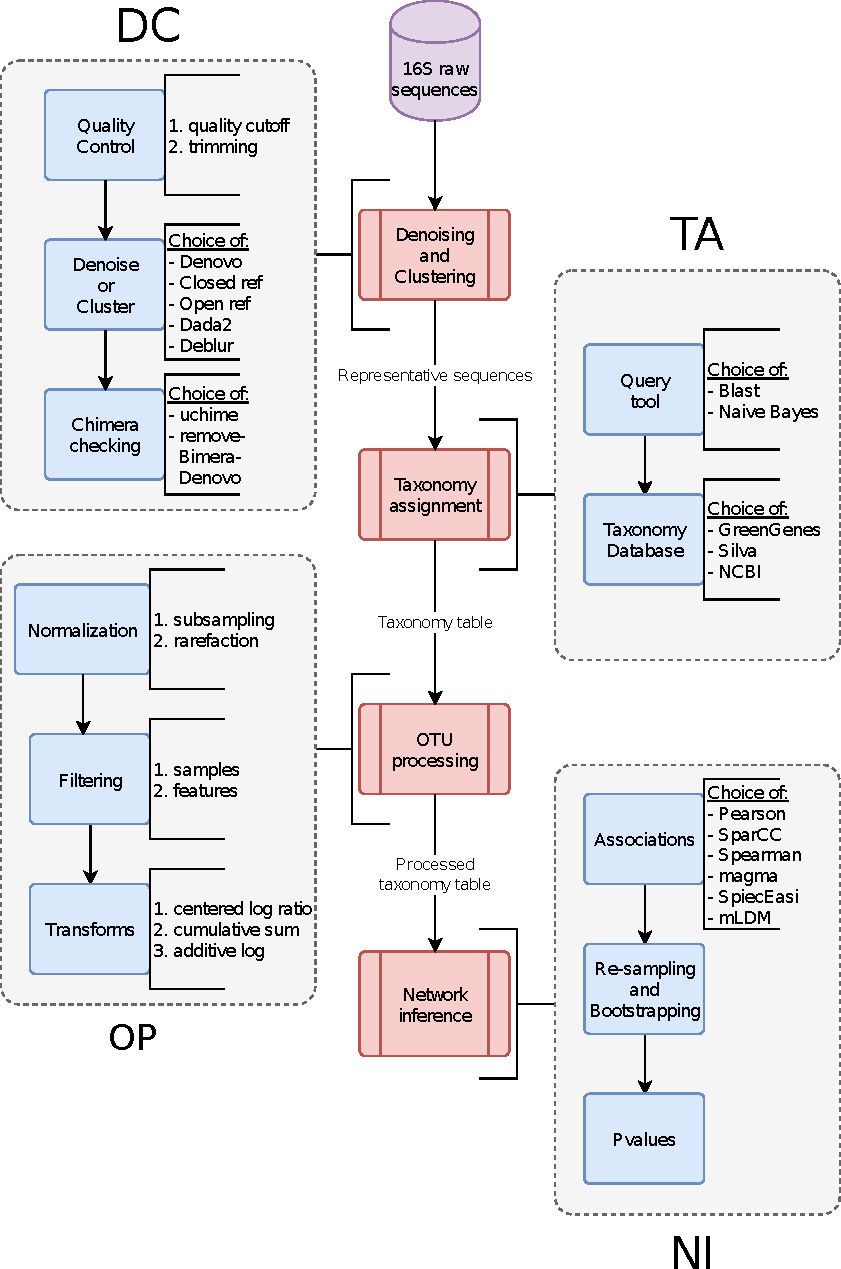
\includegraphics[width=0.7\linewidth]{figure1.pdf}
    \caption{
      \textbf{The workflow of the microbial co-occurrence analysis pipeline}.
      The processes can be grouped into four major steps: \textbf{(DC)} denoising and clustering, \textbf{(TA)} taxonomy assignment, \textbf{(OP)} OTU/ESV processing, and \textbf{(NI)} network inference.
      Each step incorporates several processes, each of which in turn have several alternate algorithms for the same task (indicated by the text to the right of the blue boxes).
      The text along the arrows describes the data that is being passed from one step to another.
    }
    \label{fig:figure1}
  \end{figure}

  % TODO: Talk about the datasets: real, mock and synthetic (with references)
  In order to objectively determine the best method we use both mock data from mockrobiota~\cite{Bokulich2016} as well as, synthetically generated reads from an Illumina read simulator called ART~\cite{Huang2012}.
  The mock datasets selected were labelled mock4, mock12 and mock16 in the mockrobiota database and consist of sequenced 16S data from mock communities of various bacteria.
  These datasets were selected since they contained the expected compositions along with the reference sequences for the organisms in the mock community.
  The synthetic reads were simulated using the three different taxonomy distribution profiles obtained from soil, water and Crohn's disease datasets.
  Reference sequences were generated using \ac{ncbi} and the decard tool \cite{Golob2017} for these taxonomy profiles.
  Detailed information on the mock communities and all the other settings used to generate the sequence data are provided in the methods section.


  \FloatBarrier

  \subsection*{The choice of reference database has the biggest impact on inferred networks}

  In order to analyze the effect of different statistical methods on the inferred co-occurrence networks, we generate co-occurrence networks using all possible combinations of methods and estimate the variability in the networks due to each choice.
  This analysis is performed while keeping the network inference algorithm the same throughout the analysis.
  The effects of various steps on the final co-occurrence network is estimated by building a linear model of the edges of the network as a function the various step in the analysis pipeline.
  Figure \ref{fig:figure2} shows the fraction of total variation among the co-occurrence networks as contributed by each of the four main steps of the pipeline.
  The 16S reference database contributes to the most variation ($\sim25\%$) in the networks, and the networks can be clearly separated based on the database used.
  This indicates that the taxonomy assigned to the reference sequences drastically alters the co-occurrence network and this change is much more significant than how the reference sequences themselves are identified (in the denoise/cluster step).
  We believe that this clustering is due to the mislabelling of constitutive taxa that are present in high abundance in the community.
  The residual variation can be seen as an artifact that arises due to the effect on the resultant network when multiple steps are changed at the same time.
  Another interesting observation has been that the dissimilarity between the networks decreases when the low abundance OTUs are removed from the network.
  These results enable us to believe that the most important criterion for accurate comparative analyses of co-occurrence networks is the taxonomy reference database.

  \begin{figure}
    \centering
    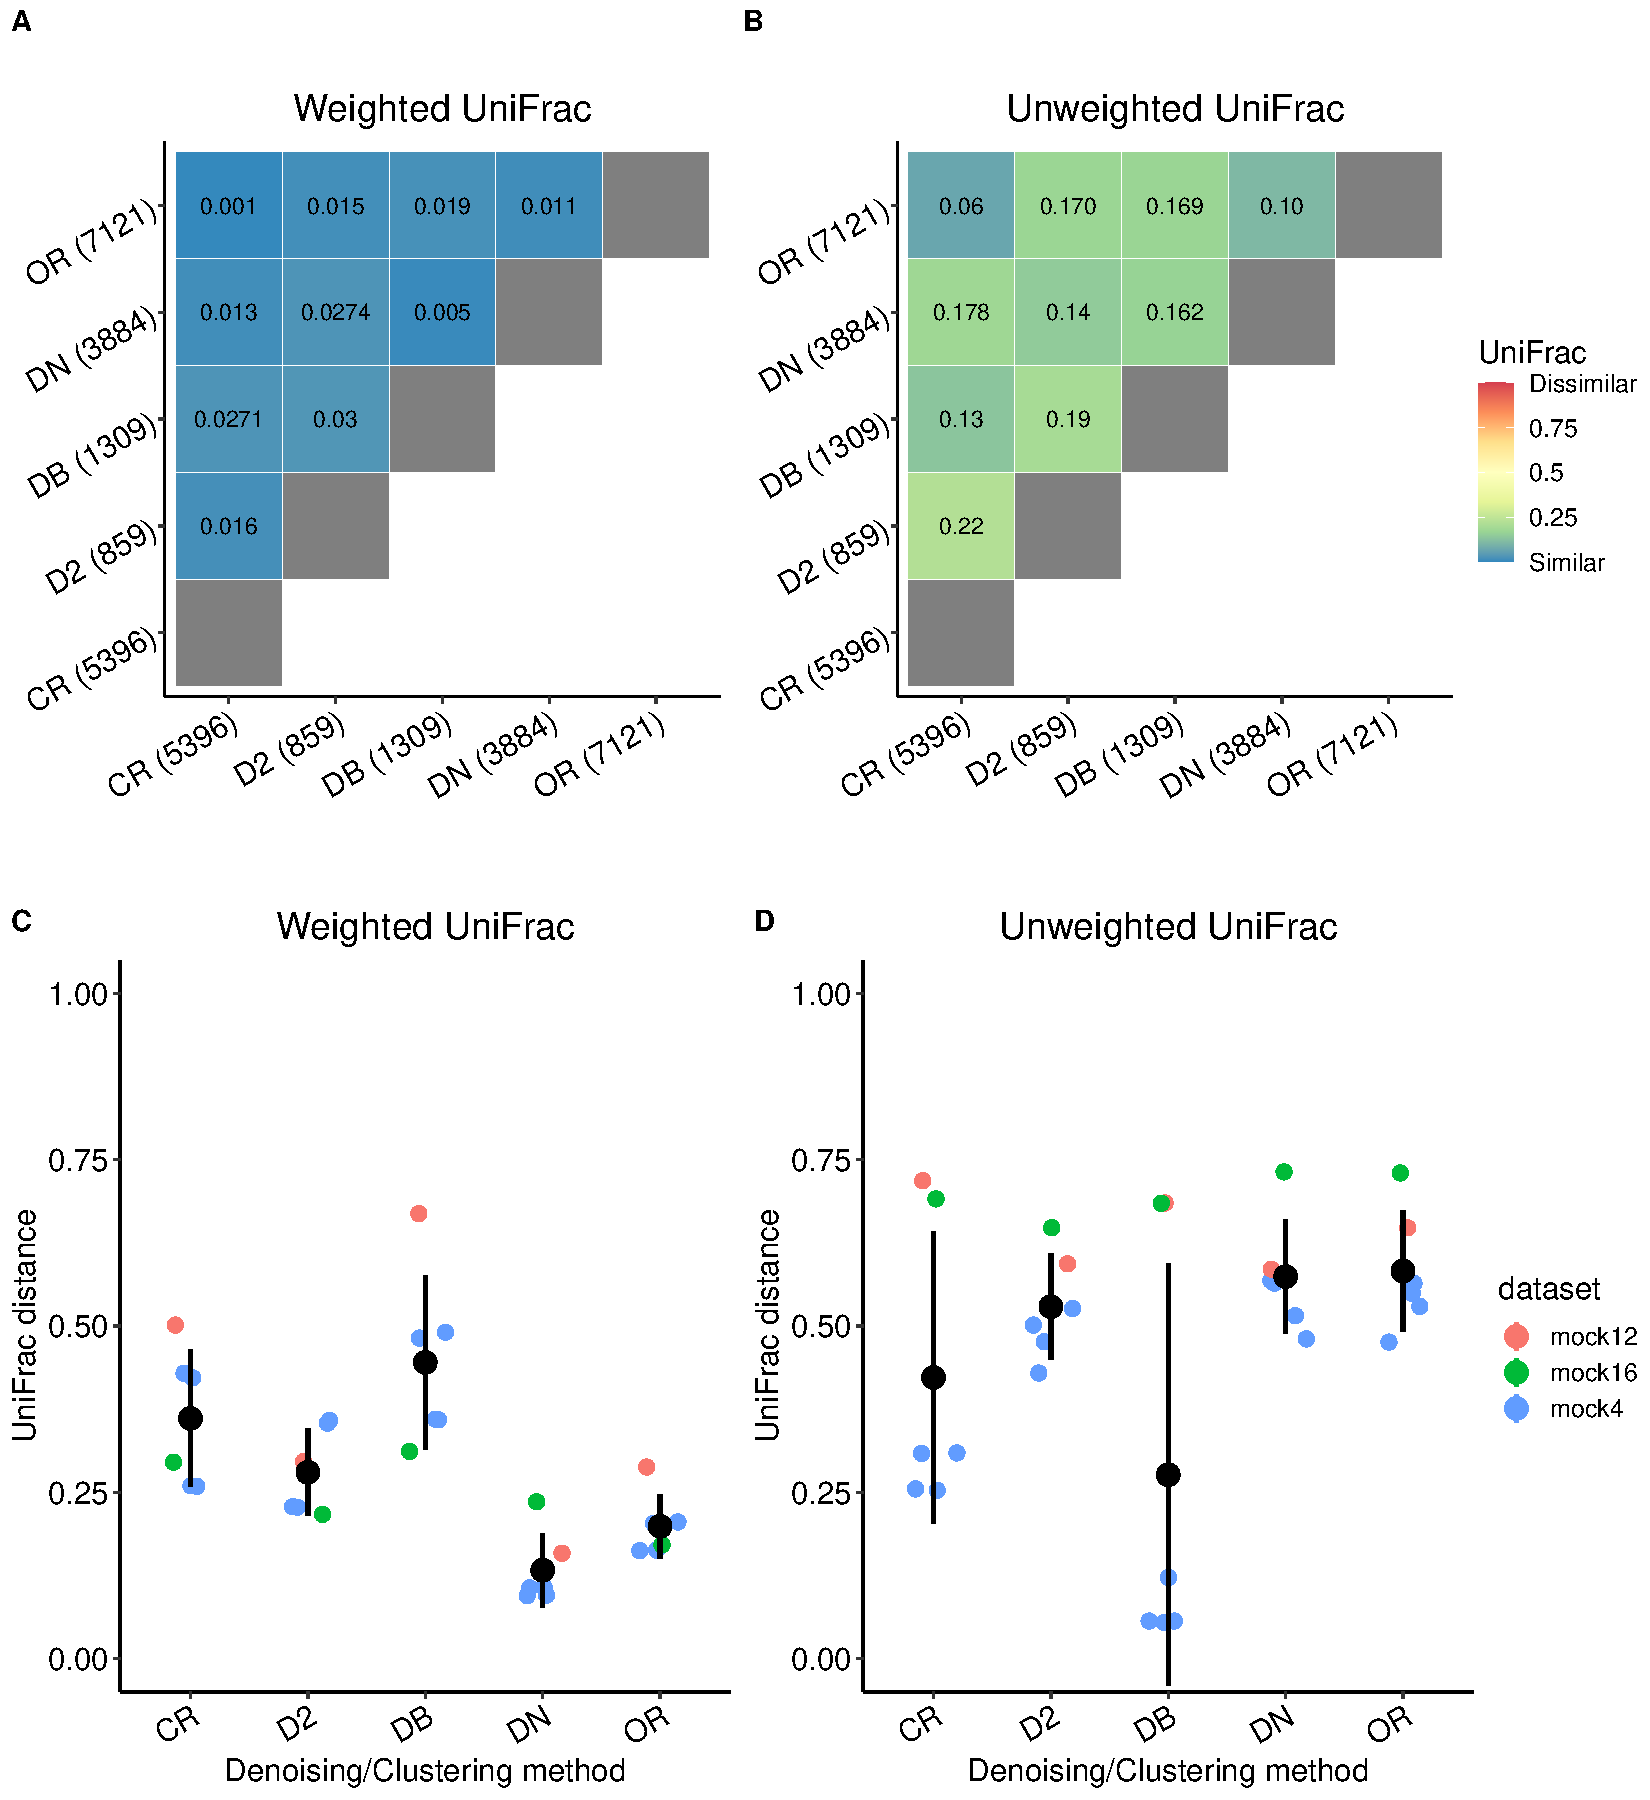
\includegraphics[width=0.85\linewidth]{figure2.pdf}
    \caption{
      \textbf{The choice of database contributes to the most variance in the networks}.
      \textbf{(A)} The total relative variance in the networks contributed by the DC, TA and OP steps of the pipeline (right) and the linear model used to calculate the relative variance (left).
      \textbf{(B)} All combinations of inferred networks are shown as points on a PCA plot.
      The color of the points corresponds to the taxonomy database, the shape corresponds to the denoising/clustering method and the size corresponds to whether low abundance OTUs were removed or not.
      \textbf{(B inset)} The network generated using DC=dada2, TA=GG, OP=no and NI=SPARCC and represents the particular point shown (big red square).
      The plot clearly shows that the points can be separated based on the TA step and that the differences due to the DC and OP steps are not as significant.
    }
    \label{fig:figure2}
  \end{figure}

  \FloatBarrier

  \subsection*{Denoising and clustering methods differ in their identification of less common reference sequences}

  Denoising and clustering are commonly carried out to generate representative sequences from the raw 16S sequencing data and to obtain the \ac{otu}/\ac{esv} tables (counts of these representative sequences for each sample).
  In order to compare the \ac{otu} tables generated by these tools we process the same 16S sequencing reads (healthy samples from a fecal microbiome transplant study [ref]) using 5 different methods \- open-reference clustering, closed-reference clustering, denovo clustering, \ac{dada2}~\cite{Callahan2016} and Deblur~\cite{Amir2017}.
  The first three methods are from the \ac{qiime1}~\cite{Caporaso2010} package.
  We find that there is good agreement in the \ac{otu}/\ac{esv} tables when different combinations of methods are used to generate them.

  To compare the representative sequences generated by these methods we employ both the weighted~\cite{Lozupone2007} (Figure~\ref{fig:figure3}A) and unweighted UniFrac method~\cite{Lozupone2005} (Figure~\ref{fig:figure3}B).
  The weighted UniFrac distance metric takes into account the counts of the representative sequences, whereas the unweighted UniFrac distance metric does not and hence gives equal weights to each sequence.
  From Figure~\ref{fig:figure3}A we can observe that the representative sequences generated by the different methods are similar to each other when weighted by their abundance.
  Figure~\ref{fig:figure3}B on the other hand shows an increase in dissimilarity between each pair of methods suggesting that the methods might differ in the sequences of low abundance.
  In order to verify this claim, we changed the threshold for the sequence count and recalculated the weighted and unweighted UniFrac distance metrics and also looked at the number of representative sequences identified in each case (in the supplementary section).

  %% TODO: Check if this is necessary
    % For each of these methods we use the same taxonomy database (\ac{gg}) to assign taxonomies to the representative sequences.
    % We then correlate the abundances of matching taxonomies between every combination of a pair of methods (Figure \ref{fig:all_denoise_reg}).
    % The \ac{esv} tables generated by methods that perform denoising are very similar to each other $\sim0.9$ and the \ac{otu} tables generated by the clustering methods are very similar to each other $\sim0.9$, but results of denoising and clustering are highly uncorrelated with each other $\sim0.4$ (Figure \ref{fig:figureS2}).
    % The common core network (network made up of edges that are predicted by all methods) is very small compared to the total number of edges predicted by all the methods (Figure \ref{fig:denoise_network}).
    % In these results, only the denoising method was changed (database used: \ac{gg} and network inference: \ac{sparcc}).

  These comparisons only elucidate the pairwise similarity or dissimilarity of a pair of methods.
  In order to determine the tool that most accurately recapitulates the reference sequences in the samples we use the 16S sequences from the mock datasets.
  The mock community datasets were processed using all the methods and the predicted representative sequences were compared with expected representative sequences and their distribution.
  The results (Figure~\ref{fig:figure3}C and D) show that the performance of the methods are similar to each other as in the case of the real dataset, but, are very different from the expected sequence distribution.
  This result is more exaggerated in the case of the unweighted UniFrac metric where some of the datasets show a very high deviation from the expected sequences.
  These high deviations are primarily in two of the three datasets that were analyzed and show that the datasets themselves play a big role in the performance of these methods.
  This can be clearly seen in the performance (weighted UniFrac distance) of \ac{dada2} and Deblur on mock12 and mock16 datasets, where, Deblur outperforms \ac{dada2} on mock12 but the under-performs on mock16.

  There is no method that clearly outperforms the rest in all datasets.
  Based on their slightly better performance on the mock datasets, their \textit{de novo} error correcting nature and other previous studies [refs] we recommend either \ac{dada2} or Deblur for users.
  However, as a result of the unexpected poor performance of Deblur on the synthetic data, the default algorithm in the pipeline was chosen to be \ac{dada2}.

  \begin{figure}
    \centering
    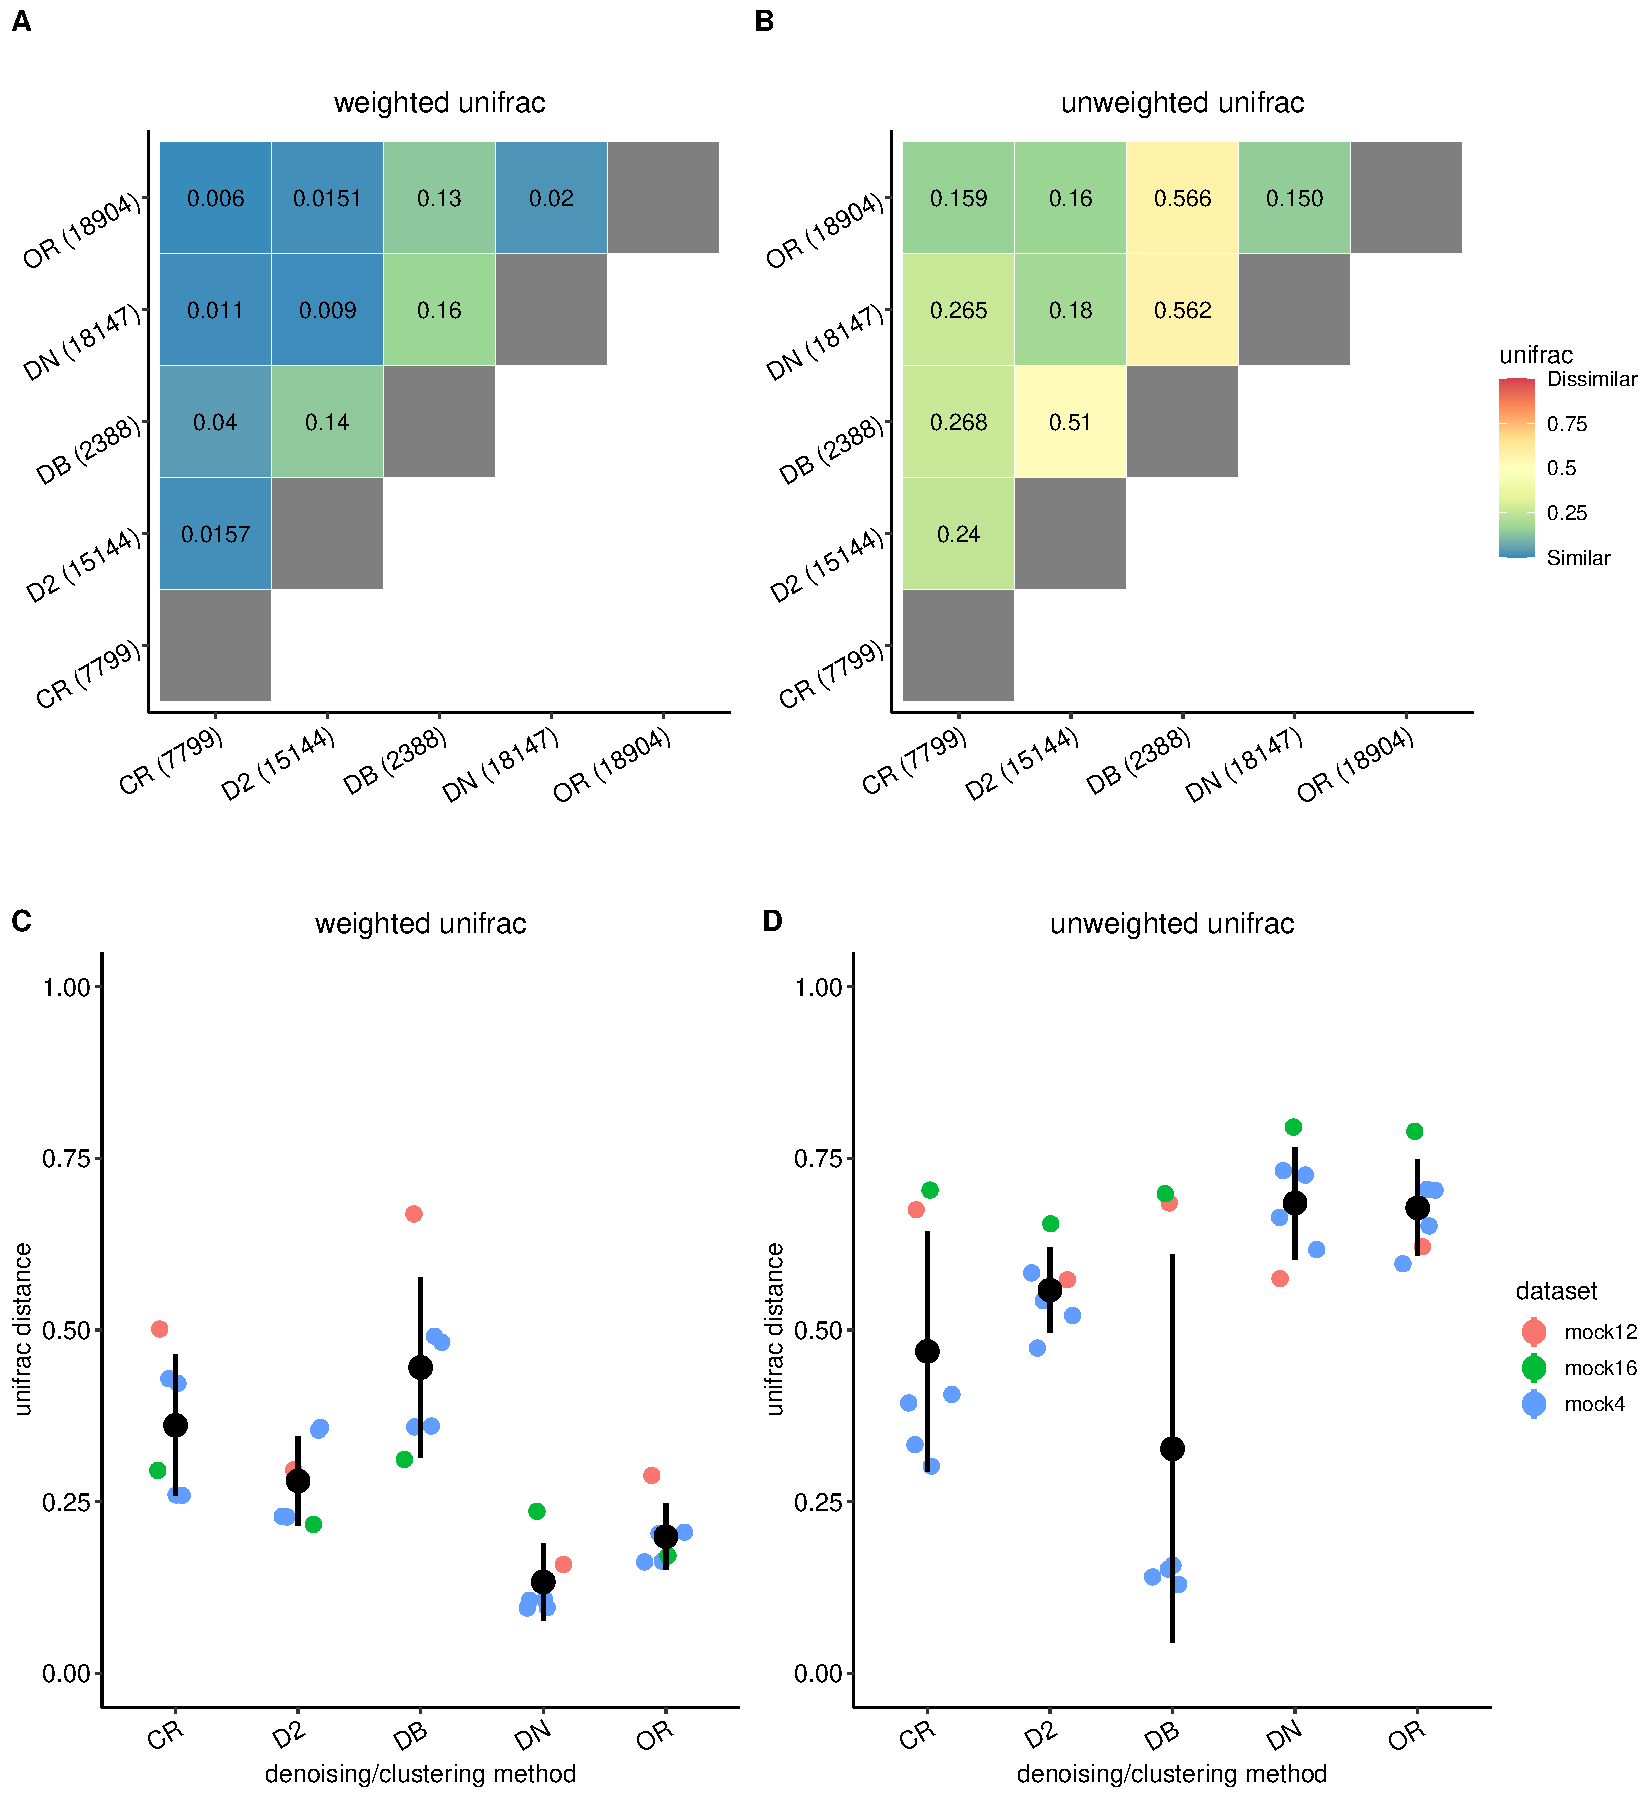
\includegraphics[width=\textwidth]{figure3.pdf}
    \caption{
      \textbf{The representative sequences generated by the different denoising/clustering methods are very similar but differ in the sequences that are in low abundance.}
      \textbf{(A)} The average weighted UniFrac distance between the representative sequences shows that the representative sequences and their compositions are fairly identical between the methods,
      \textbf{(B)} The relatively larger average unweighted UniFrac distance indicates that methods differ in their identification of sequences of low abundance,
      \textbf{(C)} The distributions of the average unweighted UniFrac distance between the expected sequence profile and the calculated sequence profile in mock datasets show that dada2 and Deblur were the best performing methods in most of the datasets.
    }
    \label{fig:figure3}
  \end{figure}

  \FloatBarrier

  \subsection*{Taxonomy databases vary widely in taxonomy hierarchy and update frequency}

  Taxonomy databases are used to assign taxonomic identities to the representative sequences obtained after the DC step.
  In order to compare the assigned taxonomies from different databases, we use the same reference sequences and assign taxonomies to them using different taxonomy reference databases.
  The three 16S taxonomic reference databases used in this study are SILVA~\cite{Quast2012}, \ac{gg}~\cite{DeSantis2006} and \ac{ncbi} RefSeq.
  SILVA and \ac{gg} are two popular 16S databases used for taxonomy identification.
  The \ac{ncbi} RefSeq nucleotide database contains 16S rRNA sequences as a part of two BioProjects - 33175 and 33317.
  The three databases vastly differ in terms of their last update status - \ac{gg} was last updated on May 2013, SILVA was last updated on December 2017 at the time of writing and \ac{ncbi} is updated as new sequences are curated.
  Since updates to taxonomic classifications are frequent, these databases vary significantly in terms of taxonomy hierarchies~\cite{Balvociute2017}.

  The representative sequences obtained from the \ac{dada2} method in DC step were used for taxonomic assignment using the three reference databases.
  Figure~\ref{fig:figure4}A depicts a flow diagram that shows how the top 50 representative sequences (sorted by abundance) are assigned a Genus according to the three different databases.
  We observe that not only does the assigned Genus composition vary significantly, but, the percentage of unassigned representative sequences (gray) also differ.
  Even the most abundant representative sequence is assigned to an "unknown" Genus in two of the three databases.
  A representative sequence might be get assigned an "unknown" Genus if either the taxonomy identifier associated with the sequence in the database did not contain a Genus or the more likely case where the database contains multiple sequences that are very similar to the query (representative) sequence and the consensus algorithm (from \ac{qiime2}) is unable to assign one particular Genus at the required confidence.
  After assigning all the representative sequences to taxonomies we perform a pairwise comparison of the similarity between assignments from different databases at every taxonomic level (Figure~\ref{fig:figure4}B).
  The assignments beyond Family level (Family, Genus and Species) are very dissimilar with $<70\%$ similarity between any pair of databases.
  There are no two reference databases that are more similar than the other, with \ac{gg} and SILVA producing only marginally similar assignments compared to \ac{ncbi}.
  This implies that the taxonomy assignments from each reference database are fairly unique and is one of the reasons for a large differences in the resultant co-occurrence networks generated from different taxonomy databases.

  As in the previous section, these comparisons only indicate similarity or dissimilarity between methods.
  In order to obtain an absolute measure of accuracy of the taxonomic assignments we use the expected reference sequences from the mock datasets as the query sequences for the databases and the expected taxonomic composition as the standard to compare against (Figure~\ref{fig:figure4}C).
  Again, we observe that none of the databases perform better than the others.

  % TODO: Check if this is necessary
    % Figure~\ref{fig:figureS3} shows that the top 20 most abundant genera in the three resulting taxonomy composition tables are different.
    % The most abundant genus in the \ac{gg} taxonomy table was \textit{Escherichia} whereas in the SILVA taxonomy table it was \textit{Escherichia-Shigella}.
    % These might seem like minor differences, but when comparing a large number of composition tables these problems are hard to diagnose.
    % Figure~\ref{fig:tax_comparison_all} shows that the result is very similar when you look at all genera instead of just the top 20 most abundant genera.
    % Moreover, Figure~\ref{fig:venn_tax} shows that there does not seem to exist a correlation between abundance and mismatch.
    % This implies that the most abundant sequences are not necessarily the ones that are consistently matched to the same taxonomies in the different reference databases.

  These results prompted us to turn to \ac{ncbi} for taxonomy assignment.
  Our reasons for choosing \ac{ncbi} are that it is regularly maintained and updated and accuracy of the assignment is still comparable to the SILVA and \ac{gg} reference databases that are routinely used as reference databases.
  % \hl{Or combine results from multiple databases?}

  \begin{figure}[h]
    \centering
    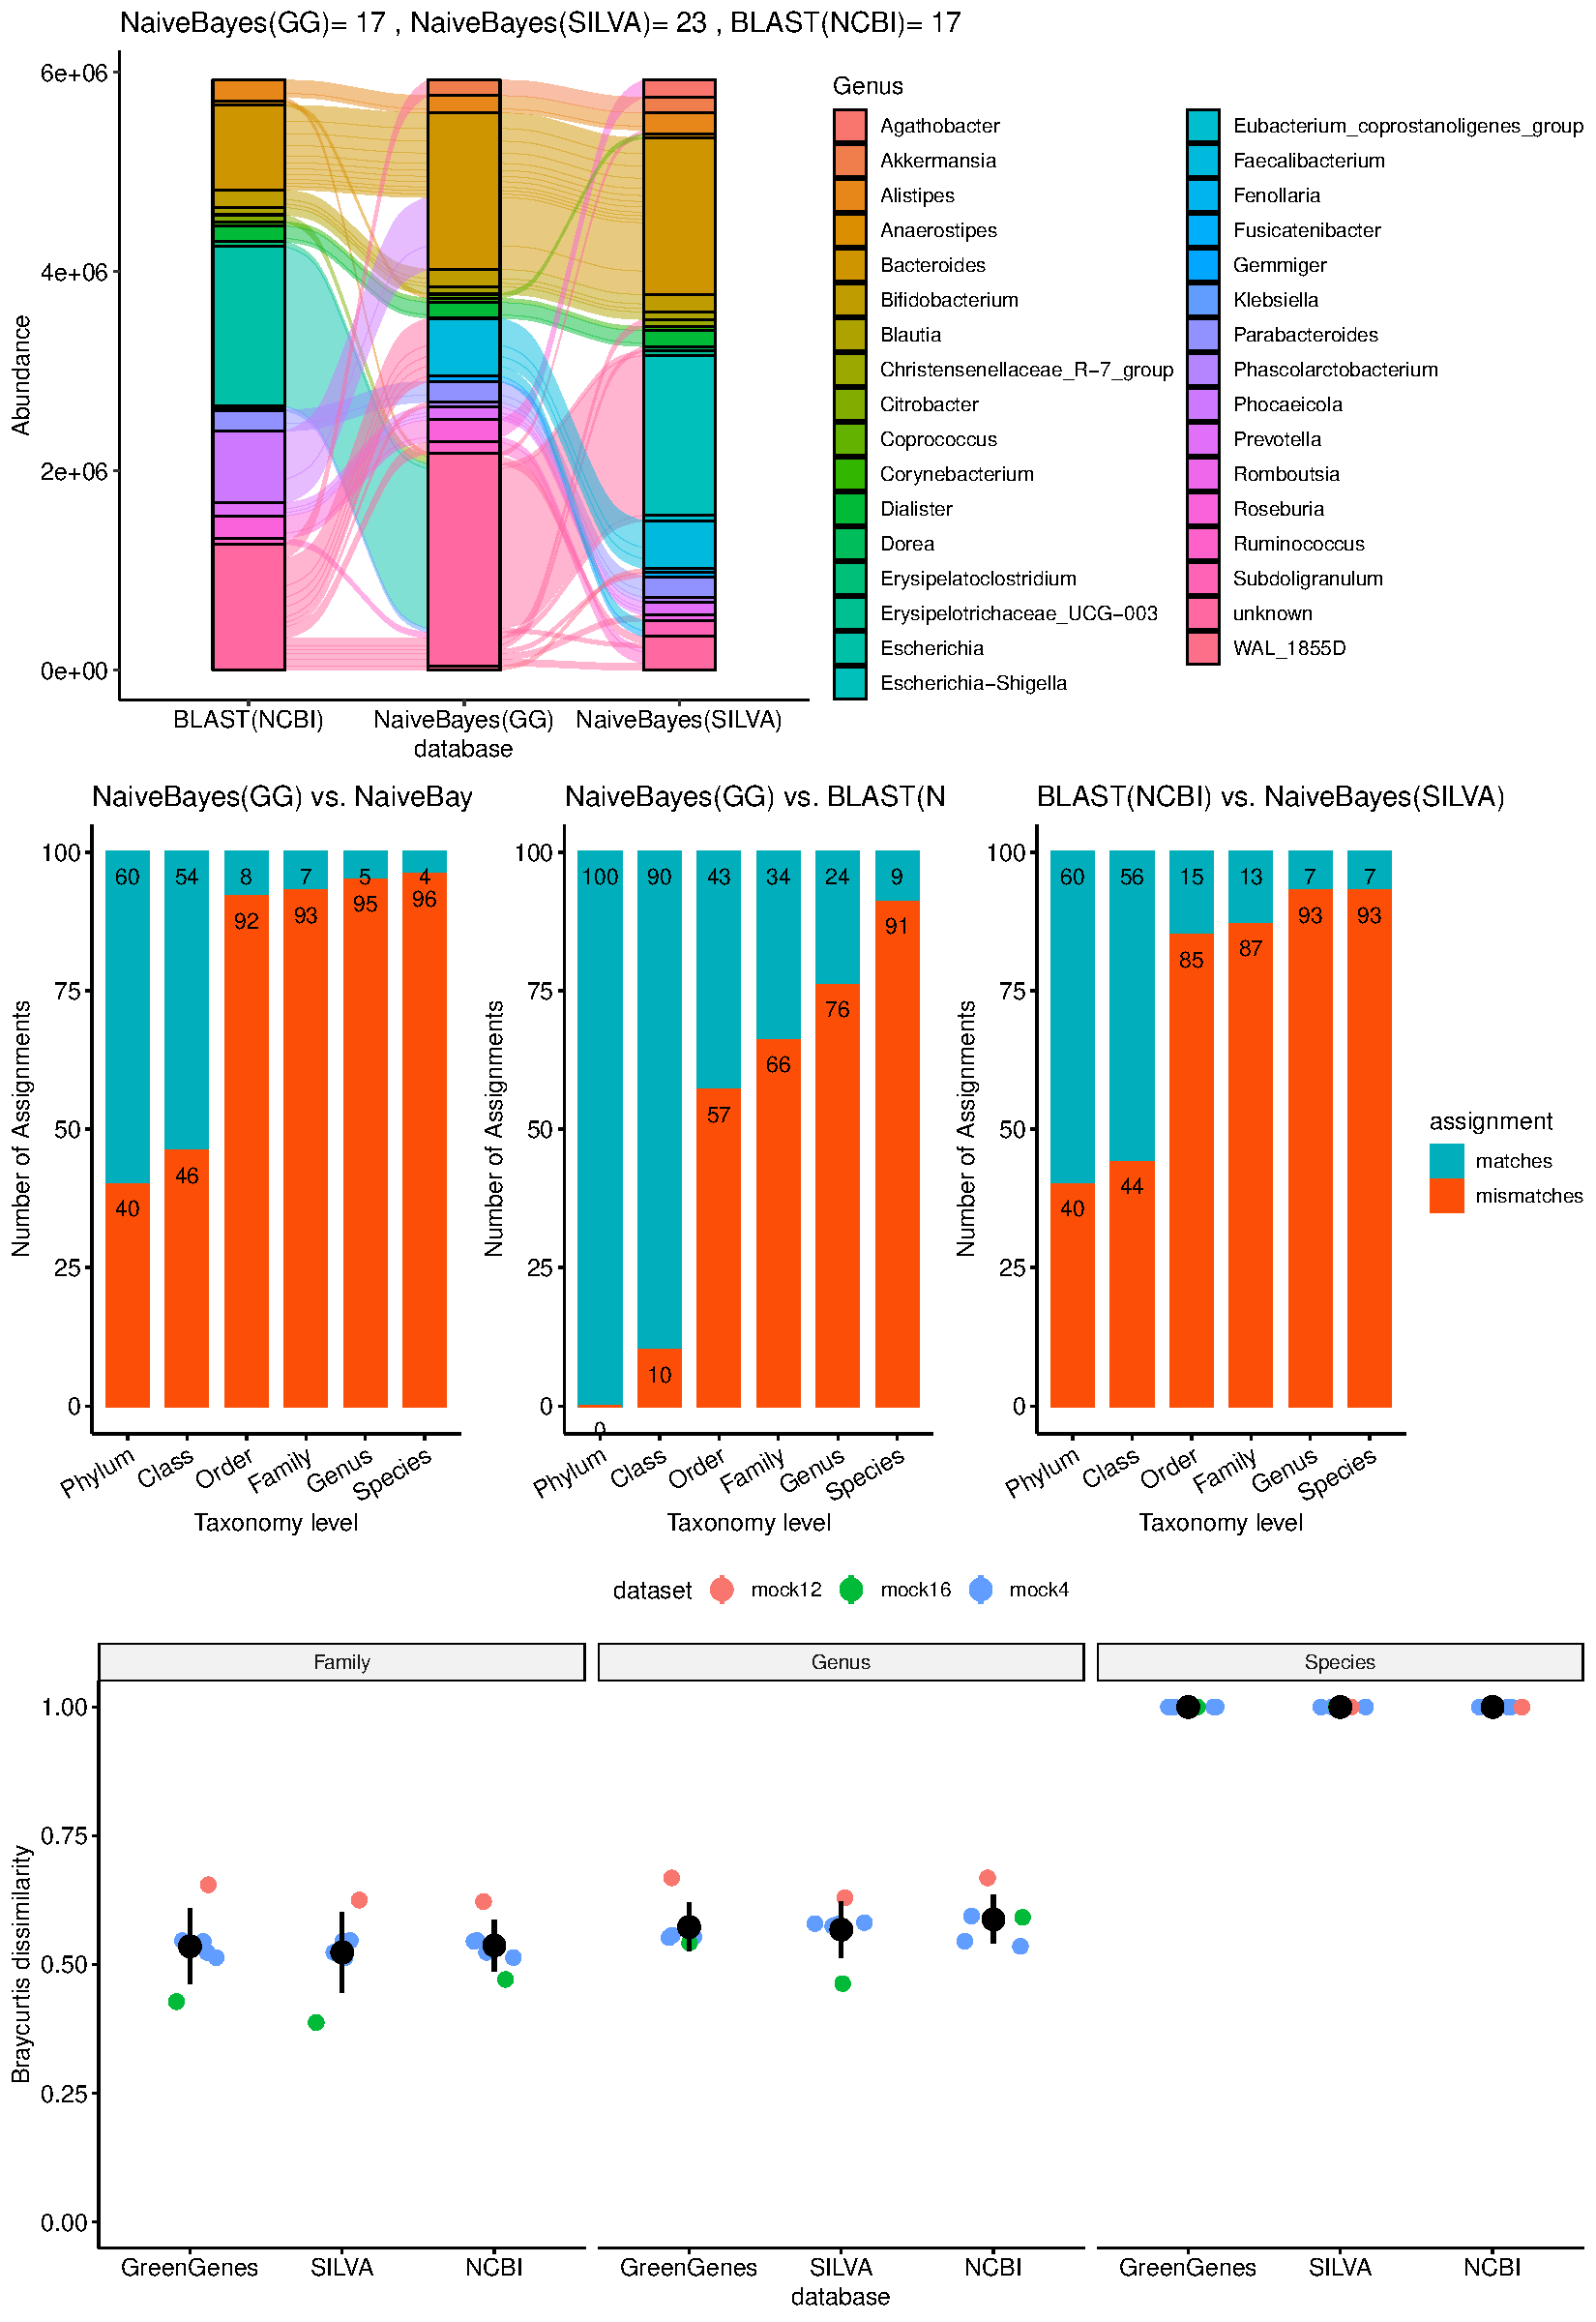
\includegraphics[width=0.72\textwidth]{figure4.pdf}
    \caption{
      \textbf{Taxonomic reference databases vary widely in terms of their taxonomy assignments.}
      \textbf{(A)} The assignment of the top 50 representative sequences to their respective taxonomies using the three different reference databases shows how the same sequences are assigned to different Genus.
      \textbf{(B)} The percentage of \ac{otu}s assigned to the same taxonomic label when using different reference databases.
      The percentage of mismatches decrease at higher taxonomic levels but even at the Phylum level there exists around 10\% of mismatches.
      \textbf{(C)} The Bray-Curtis dissimilarity between the expected taxonomy profile and calculated taxonomy profile in the mock datasets shows that there is no singular best choice of database for every dataset.
    }
    \label{fig:figure4}
  \end{figure}

  \FloatBarrier

  \subsection*{Networks generated using different network inference methods show notable difference in edge-density and connectivity}

  % TODO: Add reference here
  The six different network inference methods used in this study are \ac{magma}, \ac{mldm}, \ac{spieceasi}, \ac{sparcc}, Spearman and Pearson.
  These network inference methods into two groups, the first set of methods (Pearson, Spearman, \ac{sparcc}) infer pairwise correlations while the second set infer direct associations (\ac{spieceasi}, \ac{mldm}, \ac{magma}).

  The taxonomy composition table obtained using the \ac{ncbi} reference database is used as the input to these algorithms to infer co-occurrence associations between the microbes.
  Figure~\ref{fig:figure5}A shows the networks inferred from this dataset using the different inference algorithms.
  An edge weight threshold of 0.3 was applied to the networks generated from the methods that infer pairwise correlations and no threshold was applied in case of the other networks.
  We can clearly see that the different networks differ vastly in their edge-density and connectivity and even some of the edges in common to these networks have their signs inverted.
  To get a more quantitative idea, we can take a look at the nodes and edges (Figure~\ref{fig:figure5}B) in common between the networks using UpSet plots (only \ac{magma}, \ac{mldm}, \ac{spieceasi}, \ac{sparcc} are used in the comparison).
  The results for the node intersections show that the networks have a large number of nodes in common ($63$ out of $67$ nodes in the smallest network - \ac{magma}) and no network possesses any unique node.
  The edge intersections in contrast show that only $19$ edges (out of $98$ edges in the smallest network - \ac{magma}) are in common between all the methods and each network has a large number of unique edges.
  These results indicate that there is a substantial rewiring of connections in the inferred networks.

  Unlike in the previous sections, where were we evaluated the performance of methods on mock datasets, there are no such datasets that contain a set of known interactions for the evaluation of the network inference algorithms.
  Therefore, we propose the construction of a consensus network (Figure~\ref{fig:figure5}C) involving \ac{magma}, \ac{mldm}, \ac{spieceasi} and \ac{sparcc} by merging the p-values generated from bootstraps of the original taxonomy composition table using the Browns pvalue combining method [ref].
  The resulting network will have weights reported by all four methods.

  \begin{figure}[h]
    \centering
    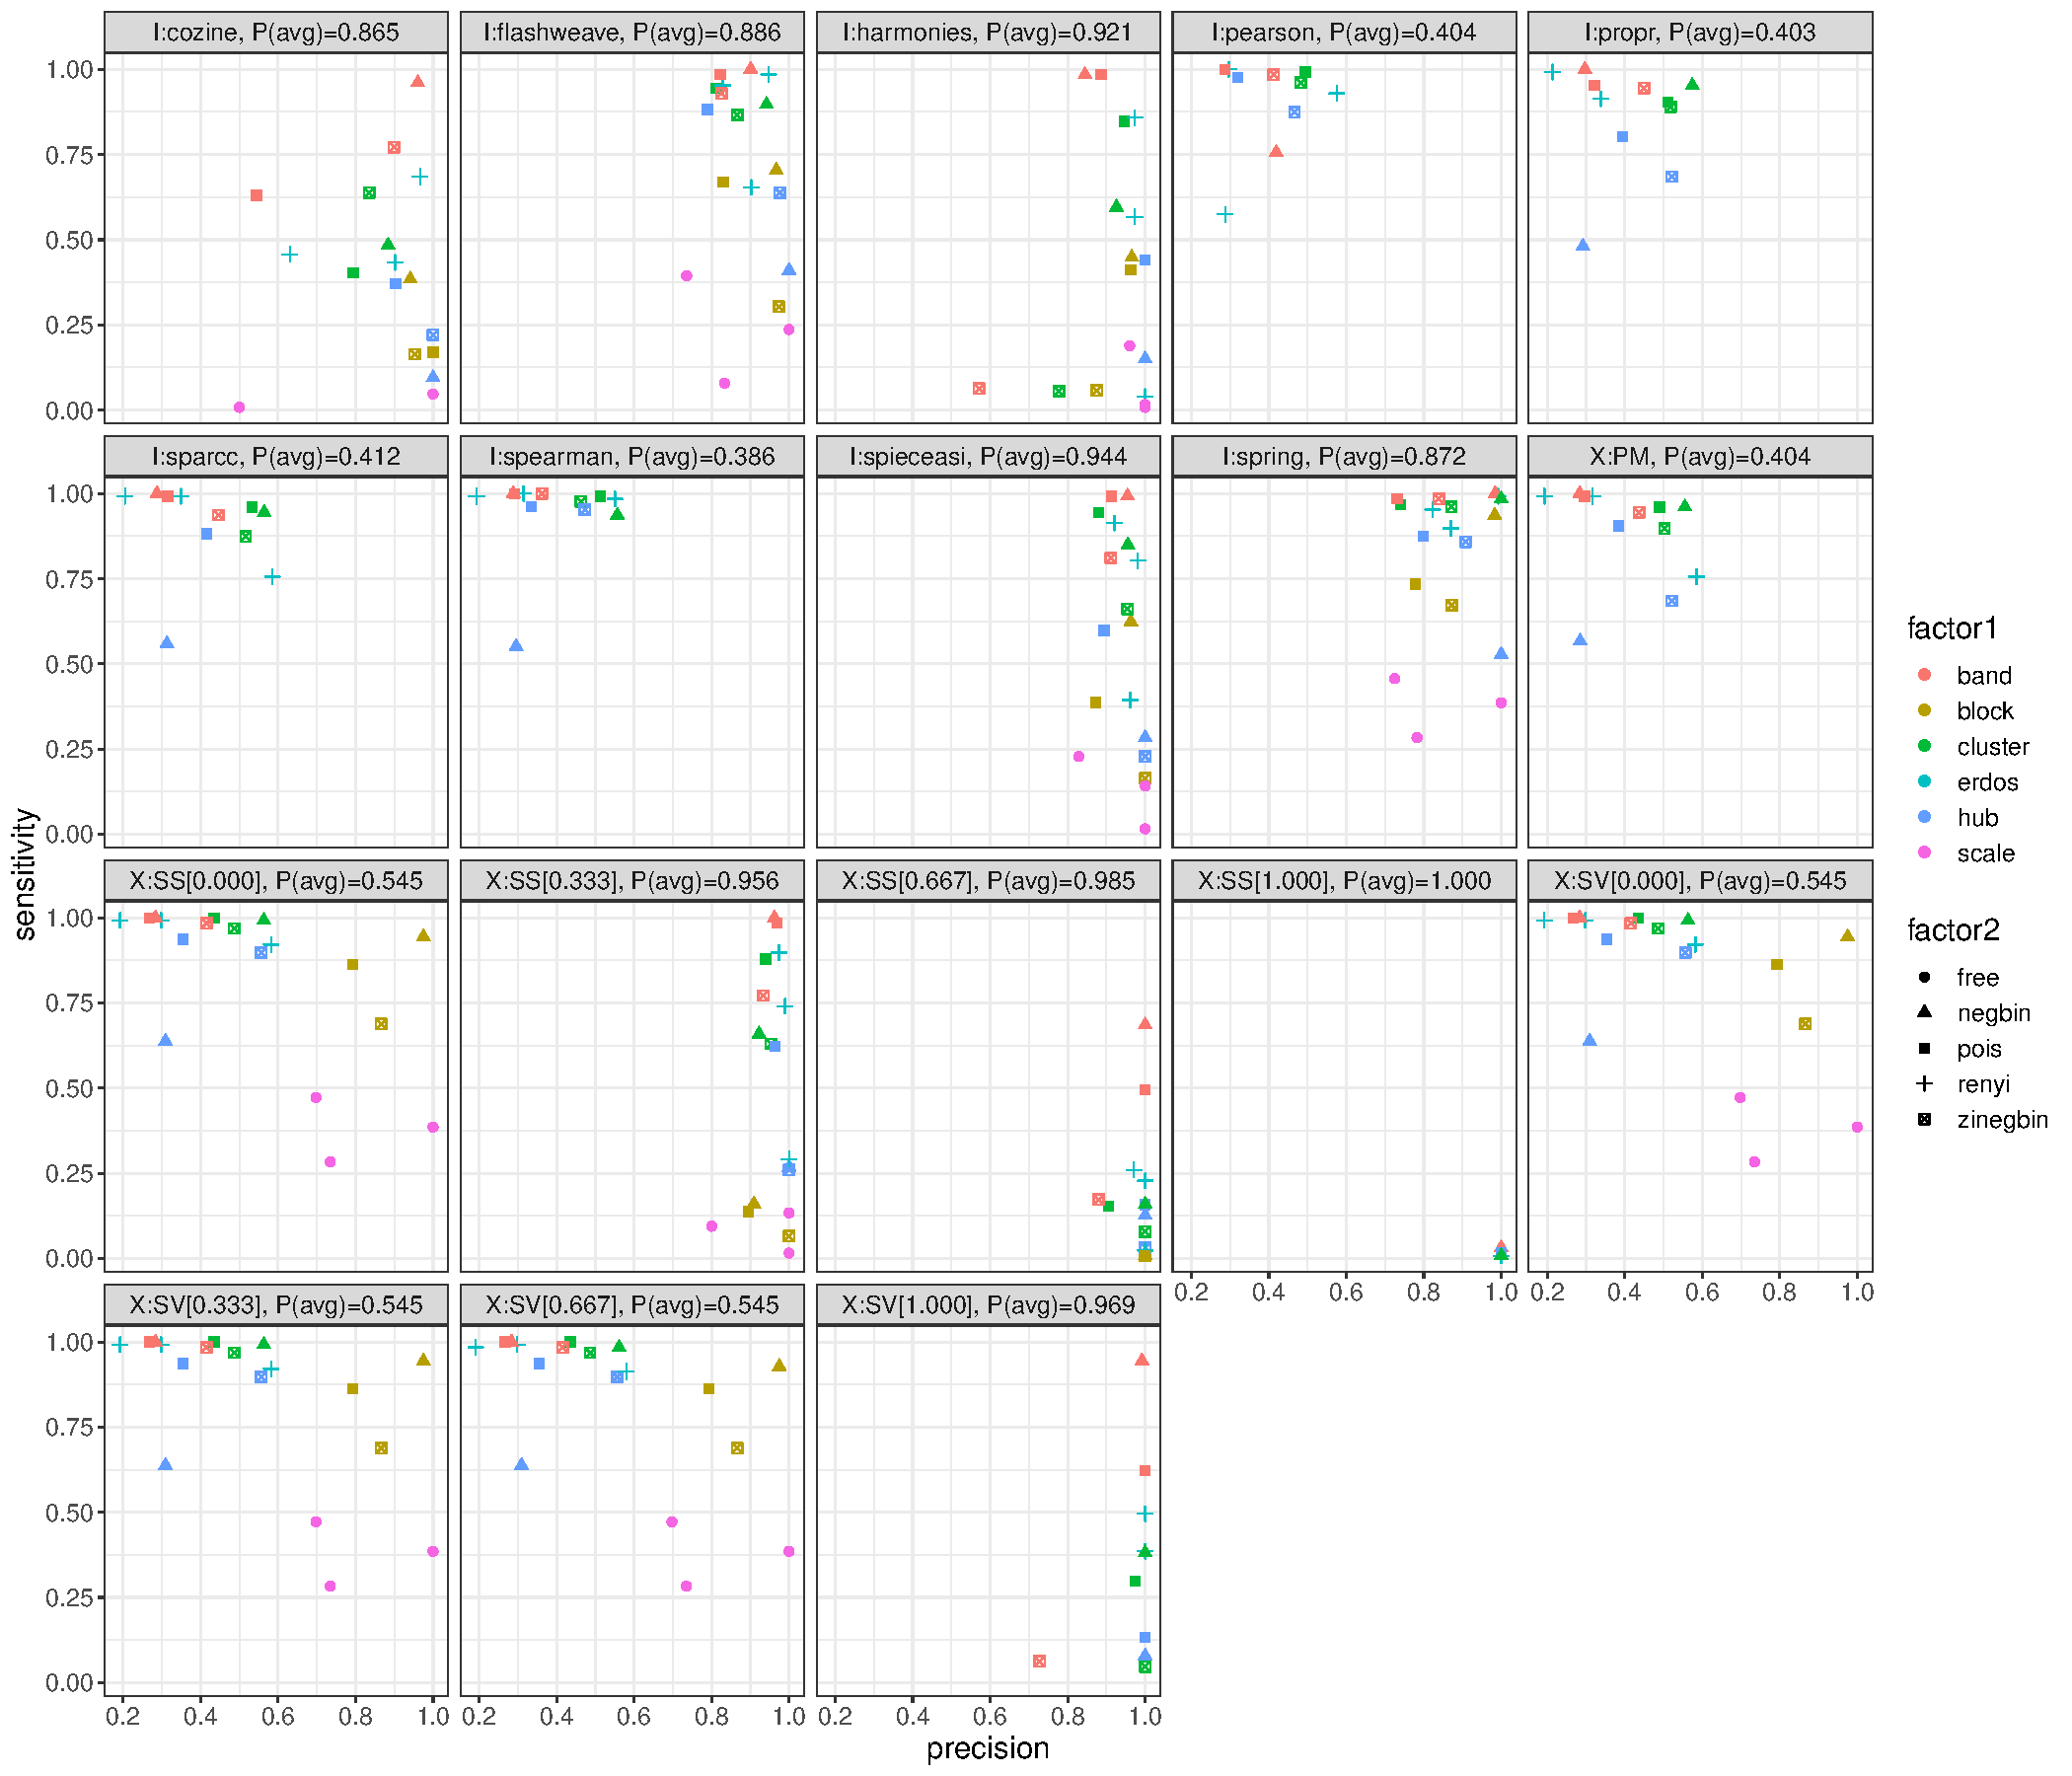
\includegraphics[width=0.85\textwidth]{figure5.pdf}
    \caption{
      \textbf{Networks generated using different network inference methods show notable differences both in terms of edge-density and connectivity}.
      \textbf{(A)} The six different networks generated by the different network inference methods are very dissimilar.
      The green links are positive associations and the orange links are negative associations.
      A threshold of 0.3 was set for the methods that infer pairwise correlations (\ac{sparcc}, Spearman, Pearson) and no threshold was set for the other methods.
      \textbf{(B)} The node overlap upset plot indicates that all the networks have a large number of common nodes involved in connections.
      Whereas, \textbf{(C)} The edge overlap upset plot shows that a very small fraction of these connections are actually shared.
    }
    \label{fig:figure5}
  \end{figure}

  \FloatBarrier

  \subsubsection*{The default pipeline}

  The systematic analysis performed in the previous sections allows us to suggest the set of tools and parameters that produce more accurate and robust co-occurrence networks.
  These tools and parameters chosen as the defaults for the pipeline and are given in Table~\ref{tab:default_options}.

  \begin{table}[h]
    \centering
    \small
    \begin{tabular}{|c|c|c|}
      \hline
      \textbf{Process} & \textbf{Tool} & \textbf{Parameters} \\
      \hline
      Denoising and Clustering & Dada2/Deblur & default \\
      Taxonomy Assignment & \ac{ncbi} with Blast & RefSeq database \\
      OTU Processing & Based on statistical power & Dynamic cutoff \\
      Network Inference & Consensus method & - \\
      \hline
    \end{tabular}
    \caption{Default tools and parameters for the pipeline}
    \label{tab:default_options}
  \end{table}

  The recommended tool for the \ac{dc} step are \ac{dada2} or Deblur were chosen based on their accuracy in recapitulating the reference sequences in mock communities and synthetic data.
  The choice of the taxonomy reference database in the \ac{ta} step is dictated largely by the species expected to be present in the sample as well the database used in similar studies if comparison is a goal.
  Nevertheless, we suggest \ac{ncbi} RefSeq along with blast+ as the query tool since the database is updated regularly and has a broad collection of taxonomies.
  The abundance threshold at the \ac{op} step is determined automatically based on the number of samples and the required statistical power.
  Finally, we use the Browns pvalue combining method on the networks generated using \ac{magma}, \ac{mldm}, \ac{spieceasi} and \ac{sparcc} to obtain a final consensus network in the \ac{ni} step.

  Figure~\ref{fig:figure6}A shows the default network compared against networks generated by altering one of the steps of the pipeline from the default.
  These results indicate that the biggest differences in networks occur when the reference database or the network inference algorithm are changed.
  Furthermore, the L1 distance of networks generated by altering one of the steps of the pipeline from the default against the default network (Figure~\ref{fig:figure6}B) show that the biggest deviations from the default network occur when the \ac{ta} and \ac{ni} steps are changed, reinforcing the same results observed in Figure~\ref{fig:figure2}. Figure~\ref{fig:figure7} shows the co-occurrence networks inferred for the hard palate for healthy subjects in a periodontal disease study [ref] and the healthy stool microbiome in fecal microbial transplant study [ref]. These consensus networks were generated using the default tools and parameters from Table~\ref{tab:default_options}.

  \begin{figure}[h]
    \centering
    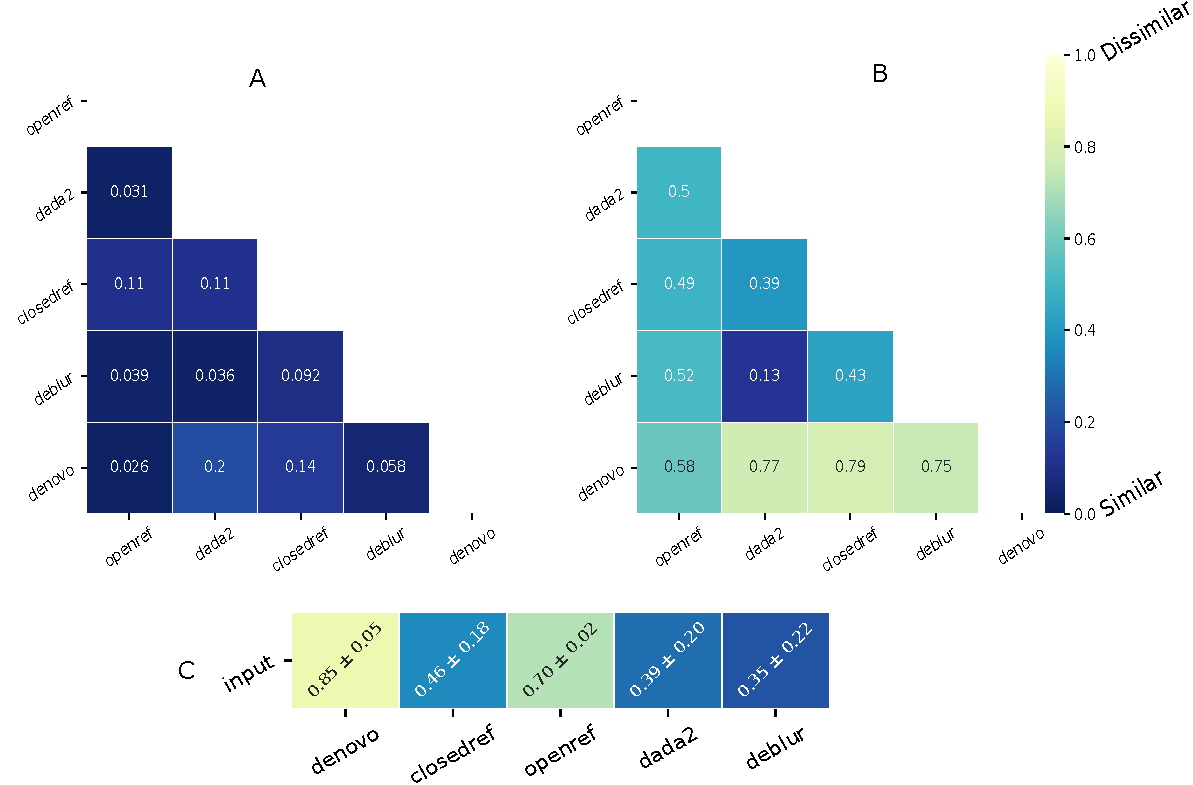
\includegraphics[width=0.9\linewidth]{figure6.pdf}
    \caption{
      \textbf{Network inference and taxonomic assignment have the highest influence on the inferred network structures.}
      \textbf{(A)} The network constructed using the default pipeline parameters (DC=\ac{dada2}, TA=\ac{ncbi}, OP=on, NI=\ac{sparcc}) is compared with networks generated when one of the steps use a different tool.
      The common connections (common with the default network) are in black, connections unique to the network are colored purple and connections in the default network but not present in the current network are gray.
      \textbf{(B)} The L1 distance between the networks generated by changing one step of the default pipeline and the network generated using the default parameters.
    }
    \label{fig:figure6}
  \end{figure}


  \begin{figure}[h]
    \centering
    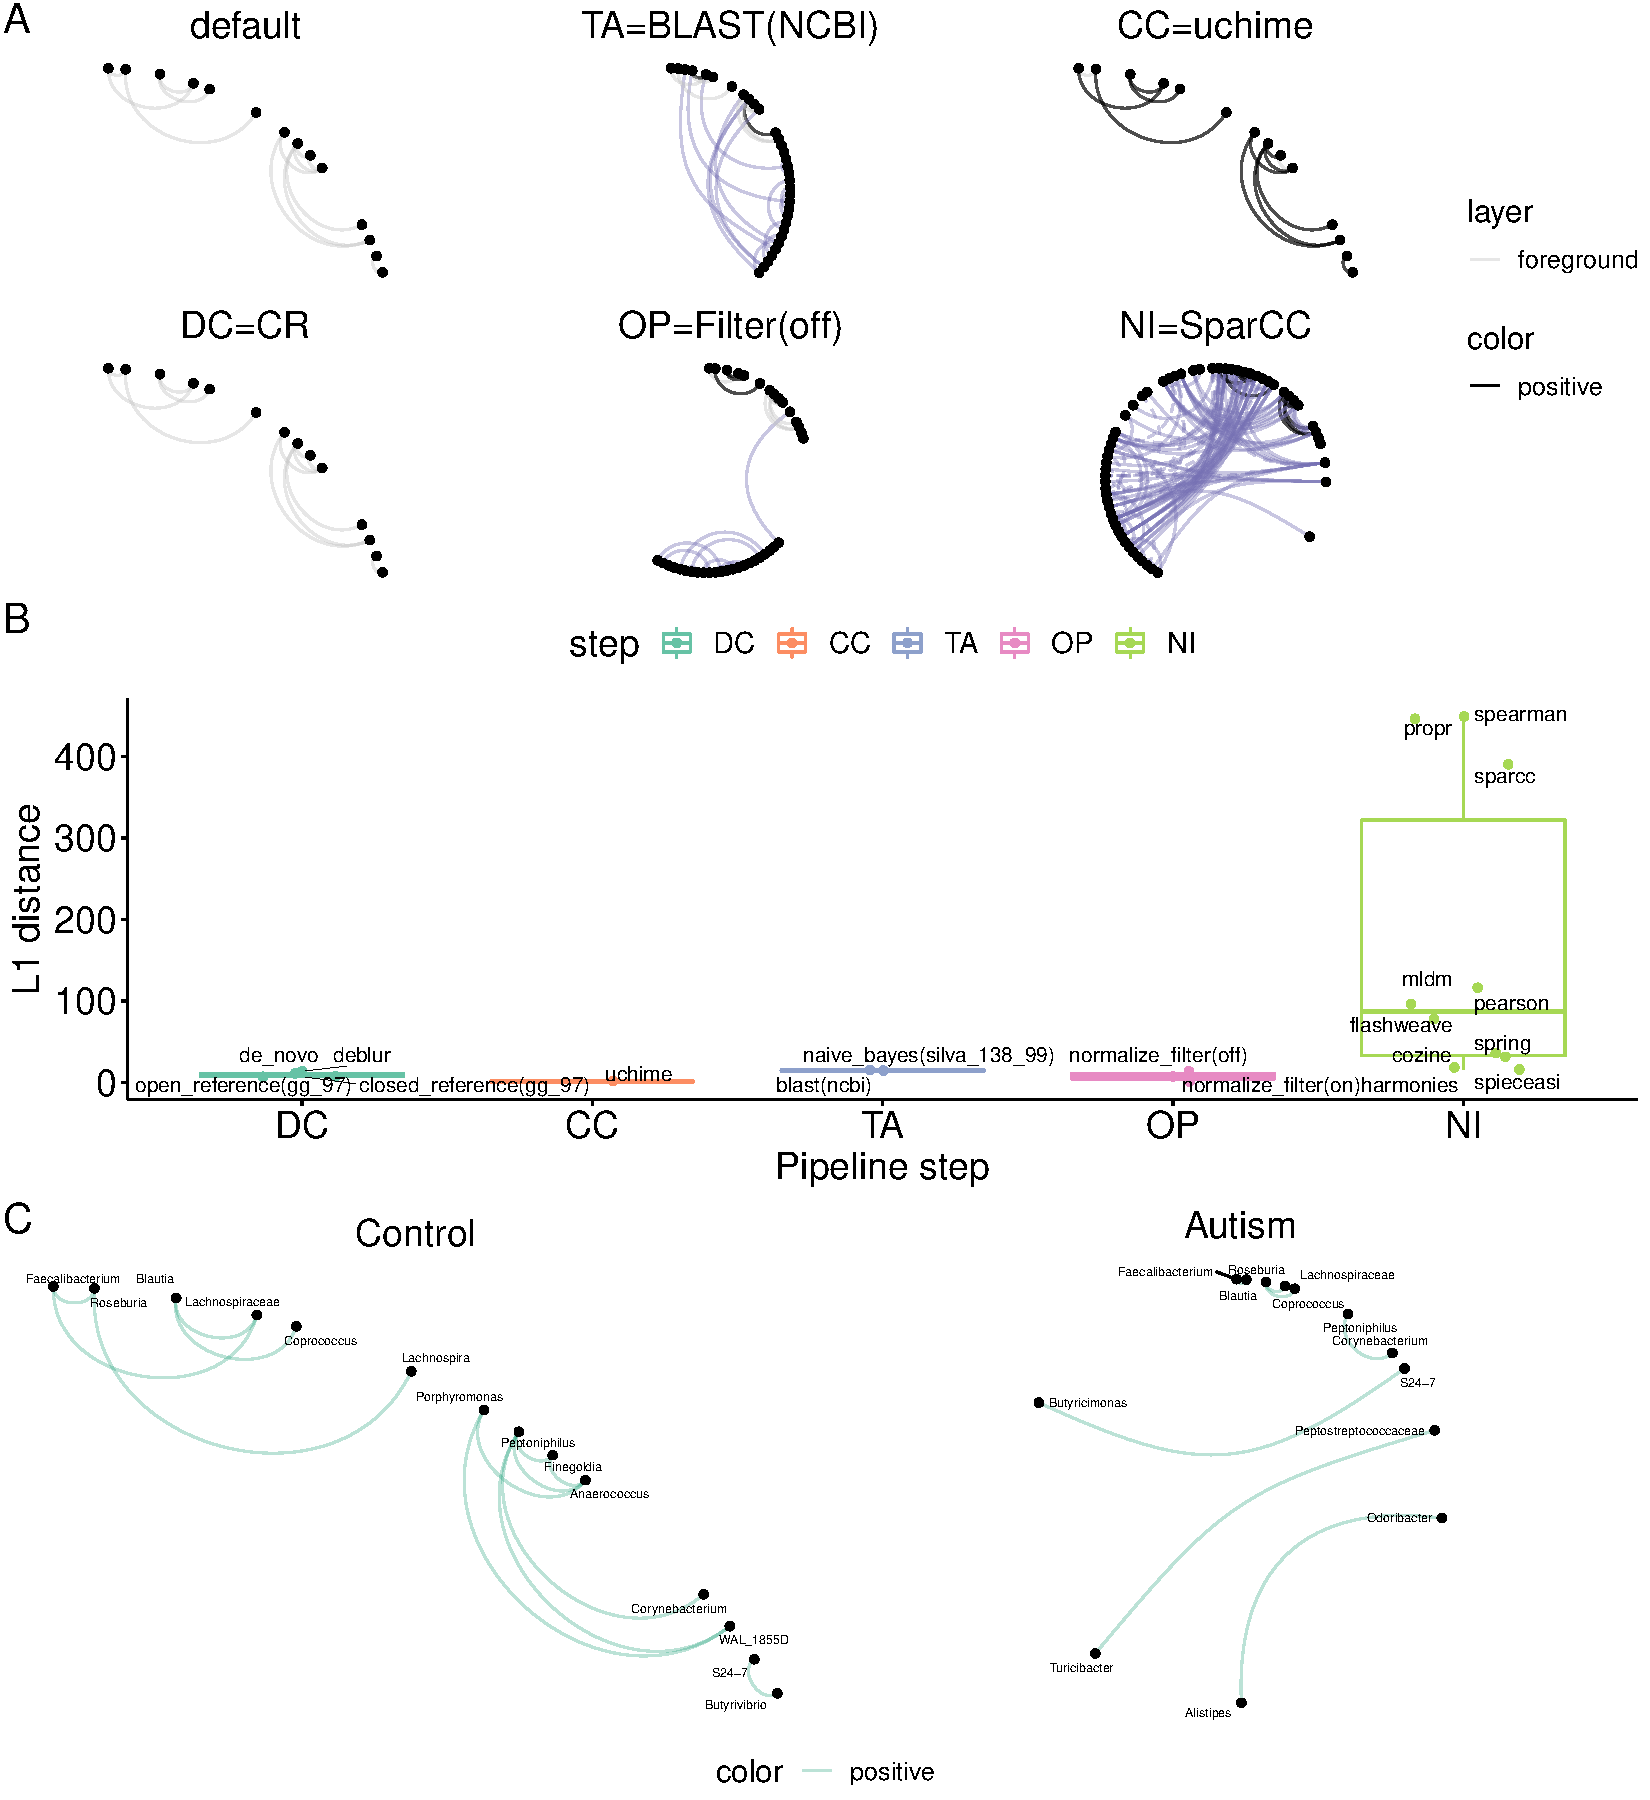
\includegraphics[width=17cm]{figure7.pdf}
    \caption{
      The consensus networks generated using the default pipeline settings.
      \textbf{(A)} Co-occurrence network of the Hard Palate microbiome generated from samples of healthy subjects in a periodontal diseases study.
      \textbf{(B)} Co-occurrence network of the Stool microbiome generated from samples of healthy subjects in a fecal microbiome transplant study.
  }
    \label{fig:figure7}
  \end{figure}
